\chapter{Manual de usuario}
\label{chap::manual}

ljksdf
fs
df

\section{Registro}

\subsection{Activación de la cuenta}

\subsection{Recuperación de la contraseña}

\section{Primer acceso}

\subsection{Las páginas de BreakBrain}

\subsubsection{Login}

Esta es la página de incio de sesión y registro. Se trata de la página que se muestra al entrar en {\tt www.breakbrain.com}.

\begin{figure}[h]
  \begin{center}
    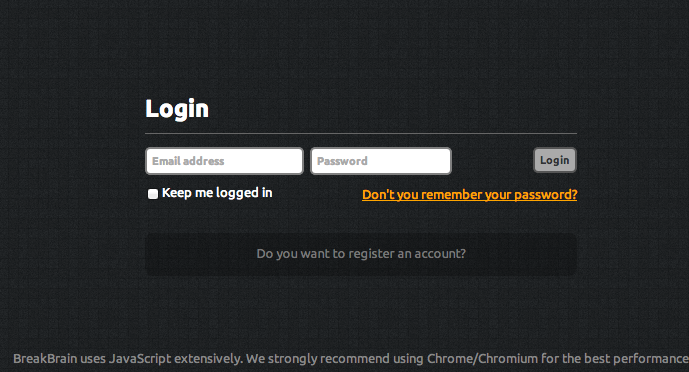
\includegraphics[width=\textwidth]{./images/page-login.png}
  \end{center}  
  \caption{Página de inicio de BreakBrain}
  \label{fig::page-login}
\end{figure}

\subsubsection{Home}

Se trata de la página principal, a la que se accede directamente iniciando sesión. En ella se ofrece un resumen breve del estado del entrenamiento cerebral, así como algunas actualizaciones de otros usuarios y los juegos recomendados.

\begin{figure}[h]
  \begin{center}
    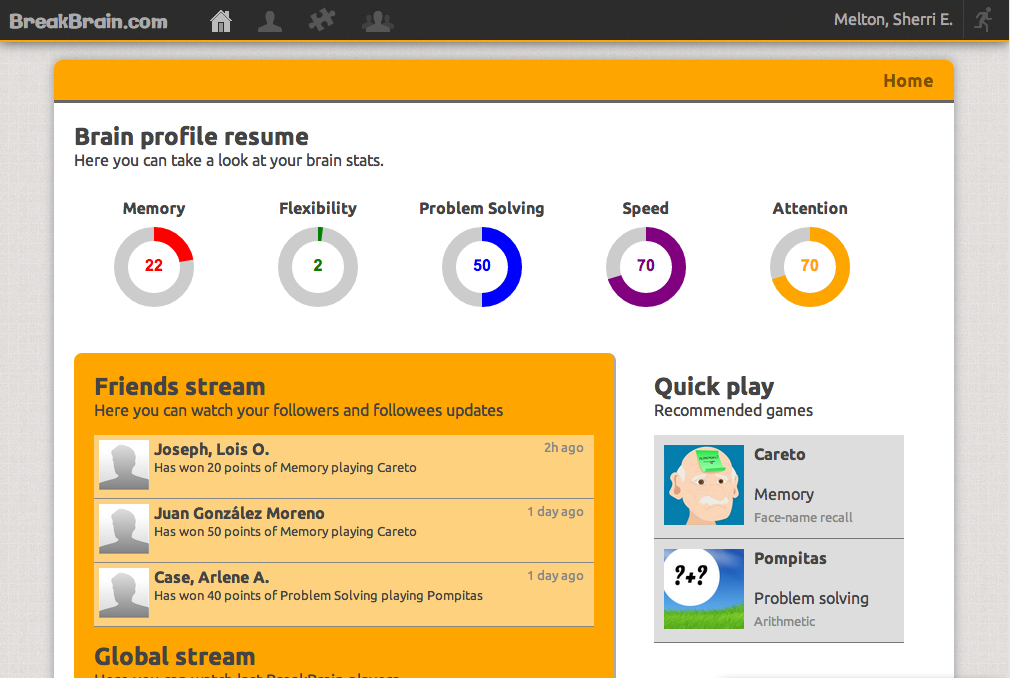
\includegraphics[width=\textwidth]{./images/page-home.png}
  \end{center}  
  \caption{Página principal de BreakBrain}
  \label{fig::page-home}
\end{figure}

\subsection{Completando el perfil de usuario}

\subsection{Definiendo las preferencias de entrenamiento}

\section{Siguiendo a otros usuarios}

\section{Entrenando el cerebro con juegos}

\subsection{Juegos monojugador}

\subsection{Jugando contra otros usuarios}
